\documentclass[twocolumn,dvipdfmx, 10pt]{article}
\usepackage{amsmath,amssymb}
\usepackage{geometry}
\usepackage[dvipdfmx]{graphicx}
\usepackage{xcolor}
\usepackage{wrapfig}
\graphicspath{{../figures/}}
\geometry{left=15mm,right=15mm,top=15mm,bottom=10mm}
\pagestyle{empty}
\begin{document}
\title{Results So Far}
\author{Neural Constructions}
\date{}
\maketitle
\thispagestyle{empty}
\subsubsection*{1.Does BERT distinguish alternating verbs and non-alternating verbs?}
We compared the verb predictions in constructions such as
\begin{center}
[SEP] the man [MASK] her the box . [SEP]
\end{center}
for DO and
\begin{center}
[SEP] the man [MASK] the box to her . [SEP]
\end{center}
for PD. The objects in these sentences were chosen for each verb.  Then, the log likelihood ratio of verb predictions in DO to those in PD is calculated:
$$\text{ln}\frac{\text{P(Verb} | \text{DO)}}{\text{P(Verb} | \text{PD)}}$$
 This ratio is expected to be smaller for non-alternating verbs since they prefer PD constructions.\\
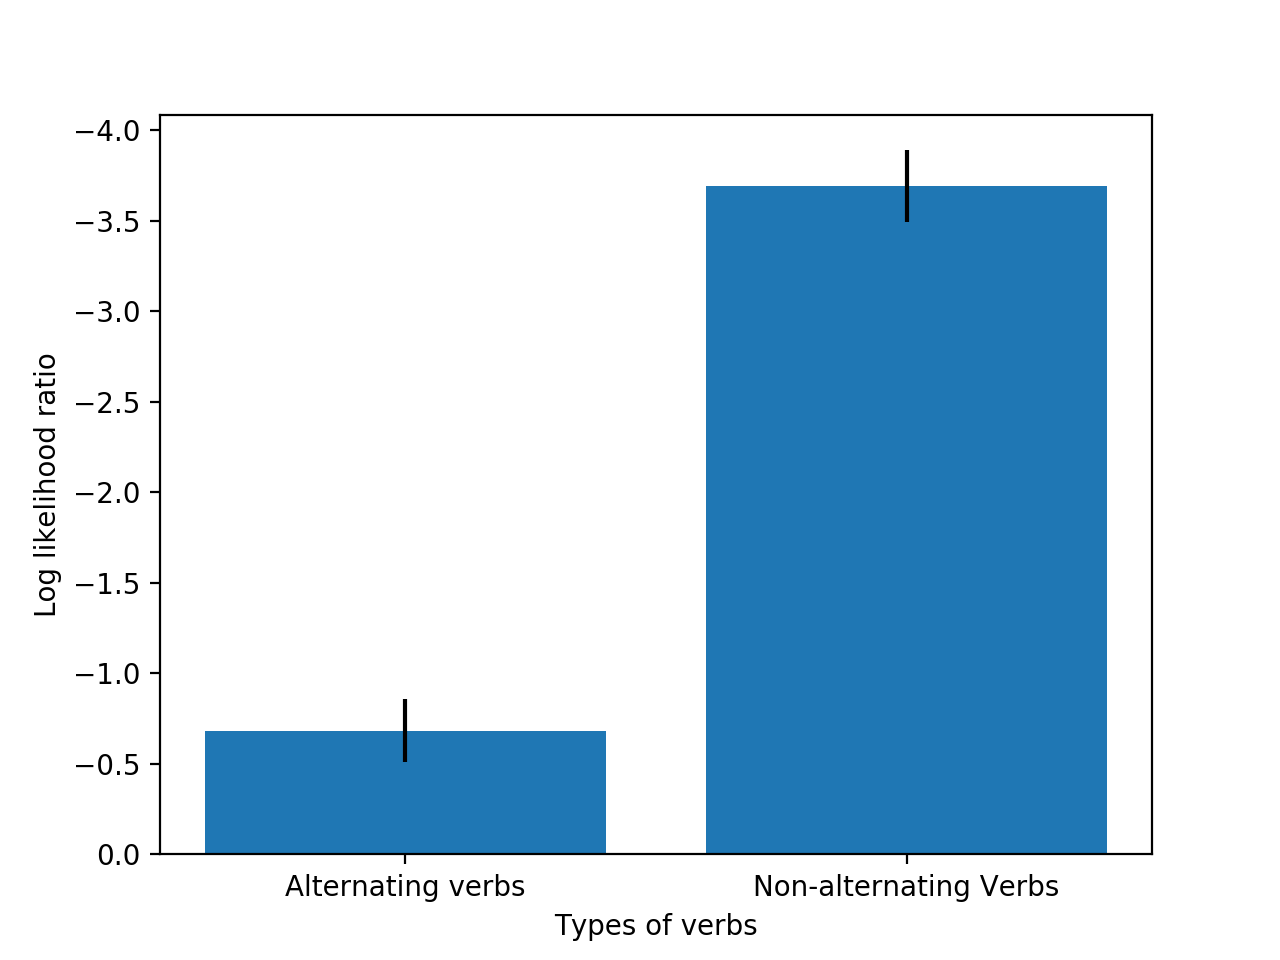
\includegraphics[keepaspectratio,width = \linewidth]{BERT.png}

\subsubsection*{2. Does BERT recognize the gradient DO preferences among verbs?}
We sorted by the log likelihood ratio for each verb and obtained the following result.\\
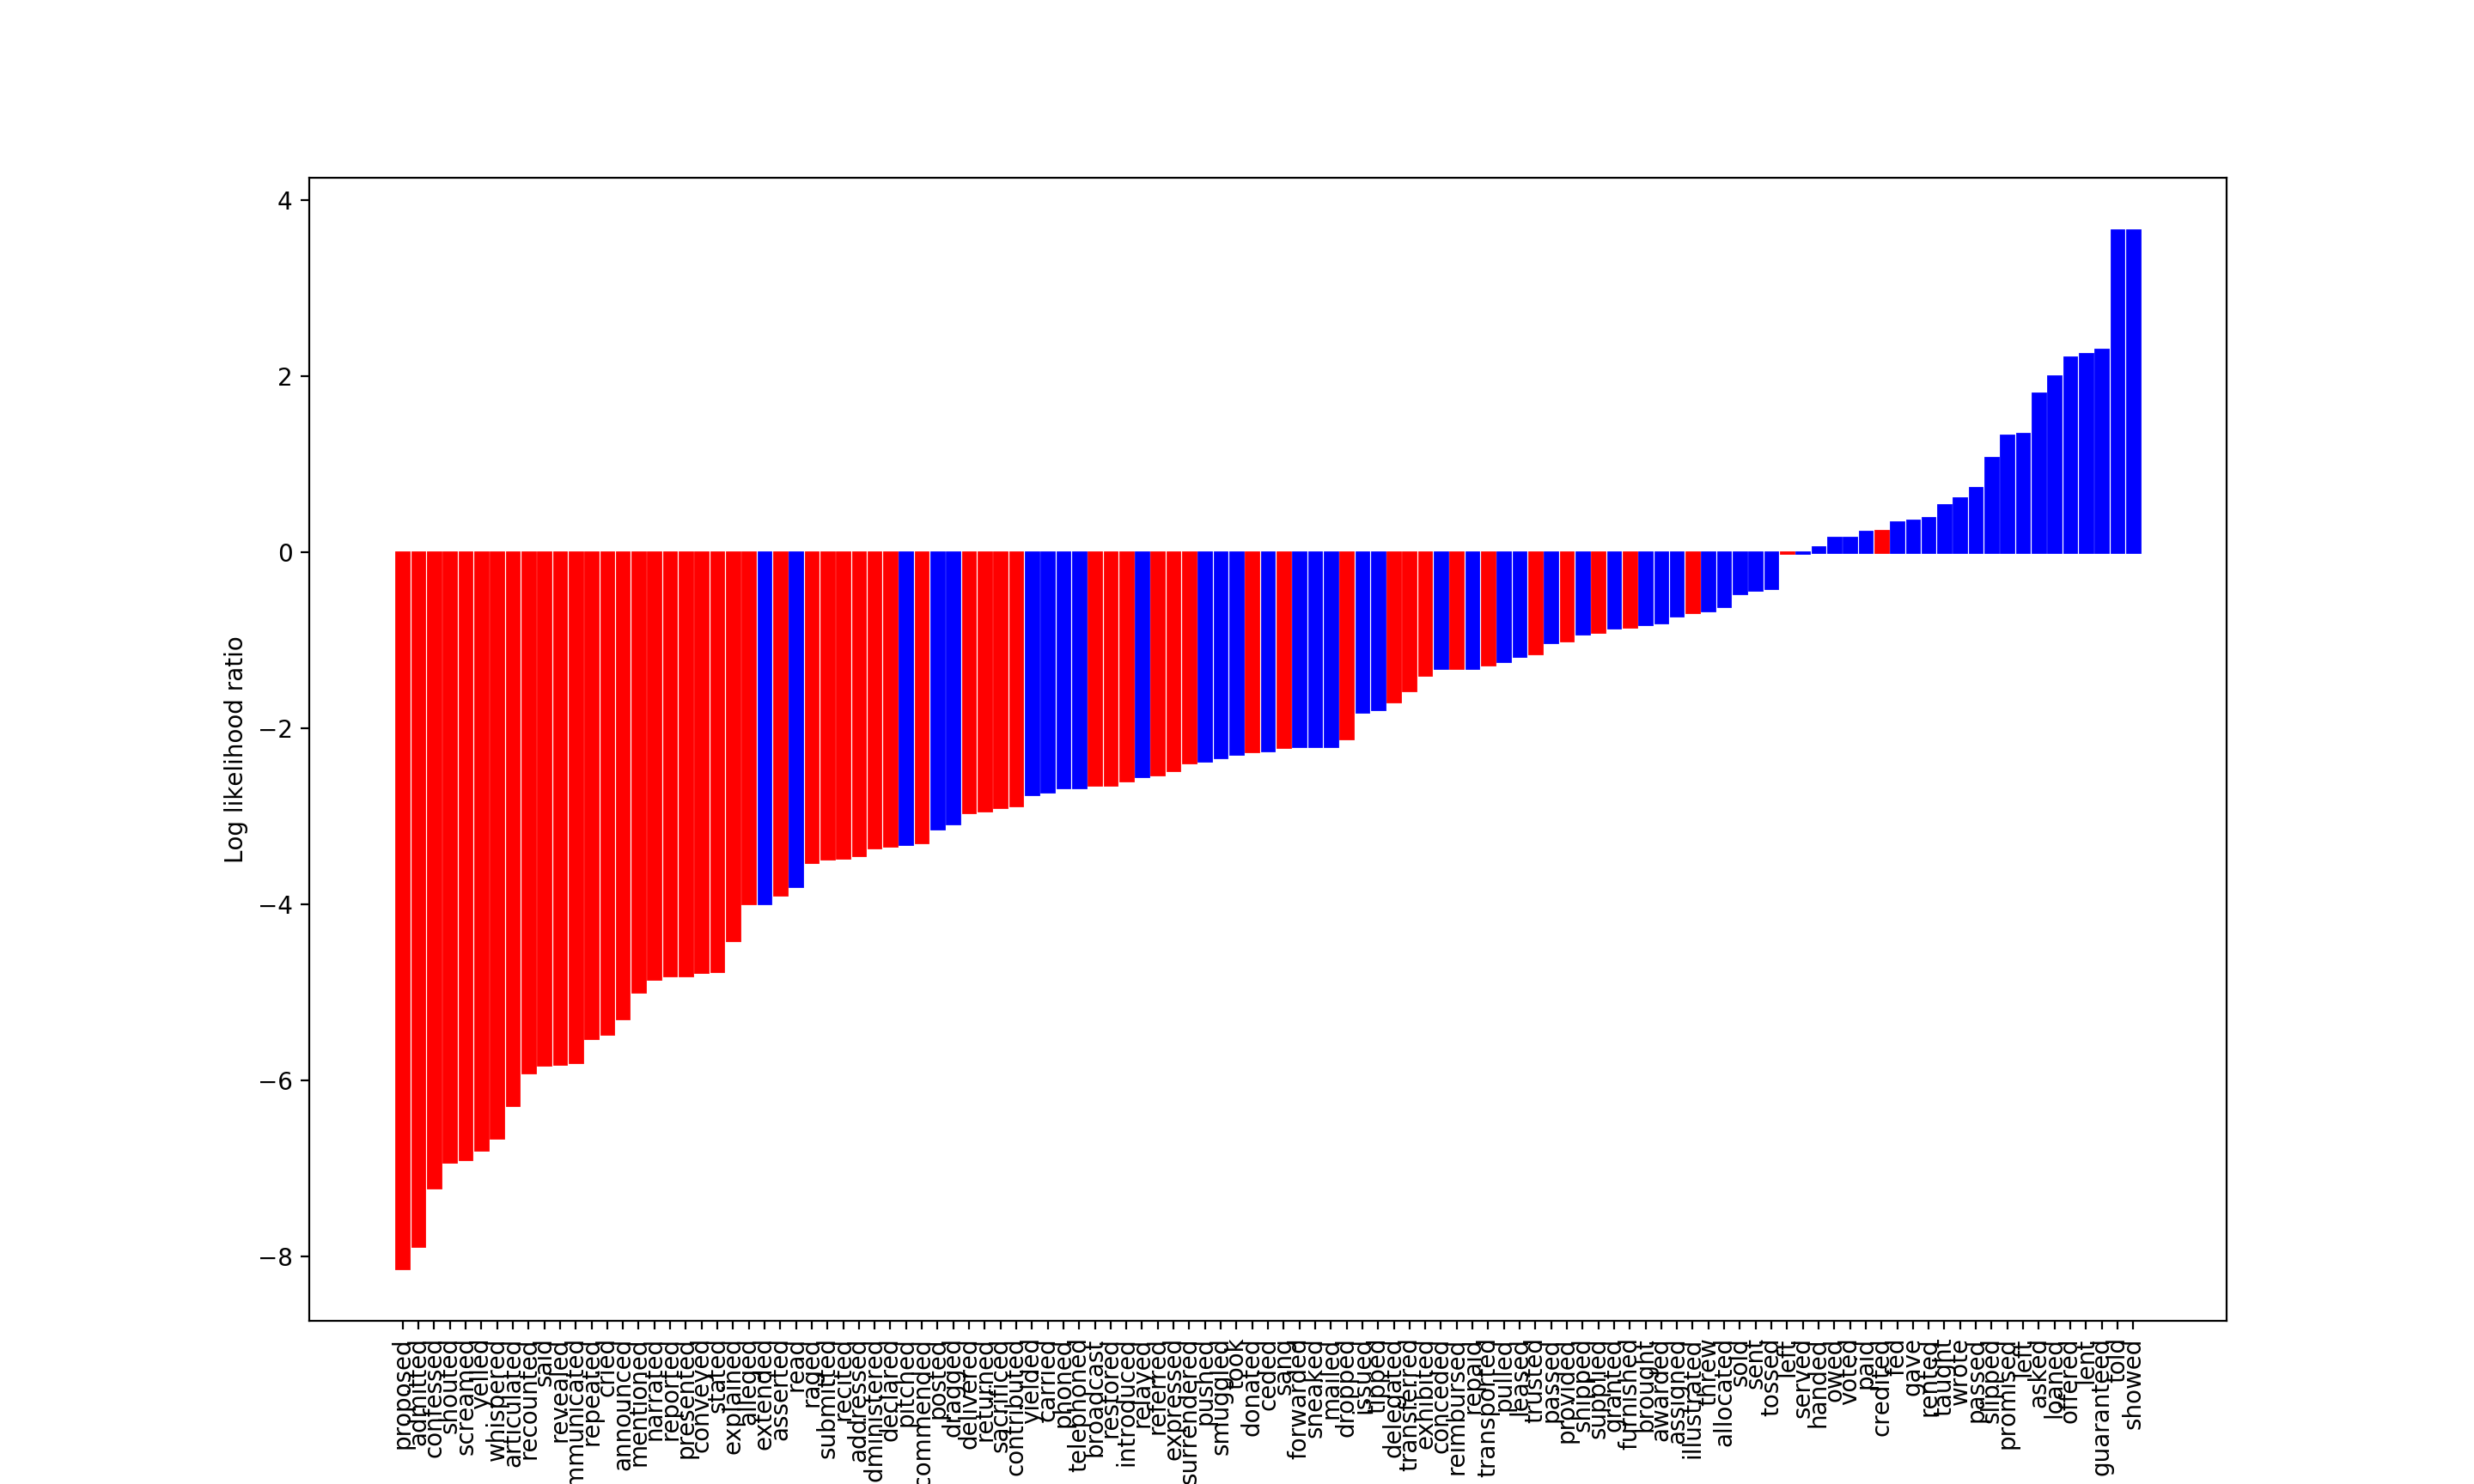
\includegraphics[keepaspectratio,width = \linewidth]{BERT_individual.png}

\subsubsection*{3. Does BERT just track transitional probability?}
In order to show that BERT does more than tracking transitional probabilities, we calculated the log probability of verb prediction
$$\text{ln}\text{P(Verb} | \text{Construction)}$$
for non-alternating verbs in the following two constructions.\\
$[$SEP$]$ the man $[$MASK$]$ her the news . $[$SEP$]$\\
$[$SEP$]$ the man $[$MASK$]$ her news to the friend . $[$SEP$]$\\
The first construction does not allow the non-alternating verb but the second one does.  If BERT just track transitional probability, it will assign low probabilities for both constructions because they share the bigram ``$[$MASK$]$ her".\\
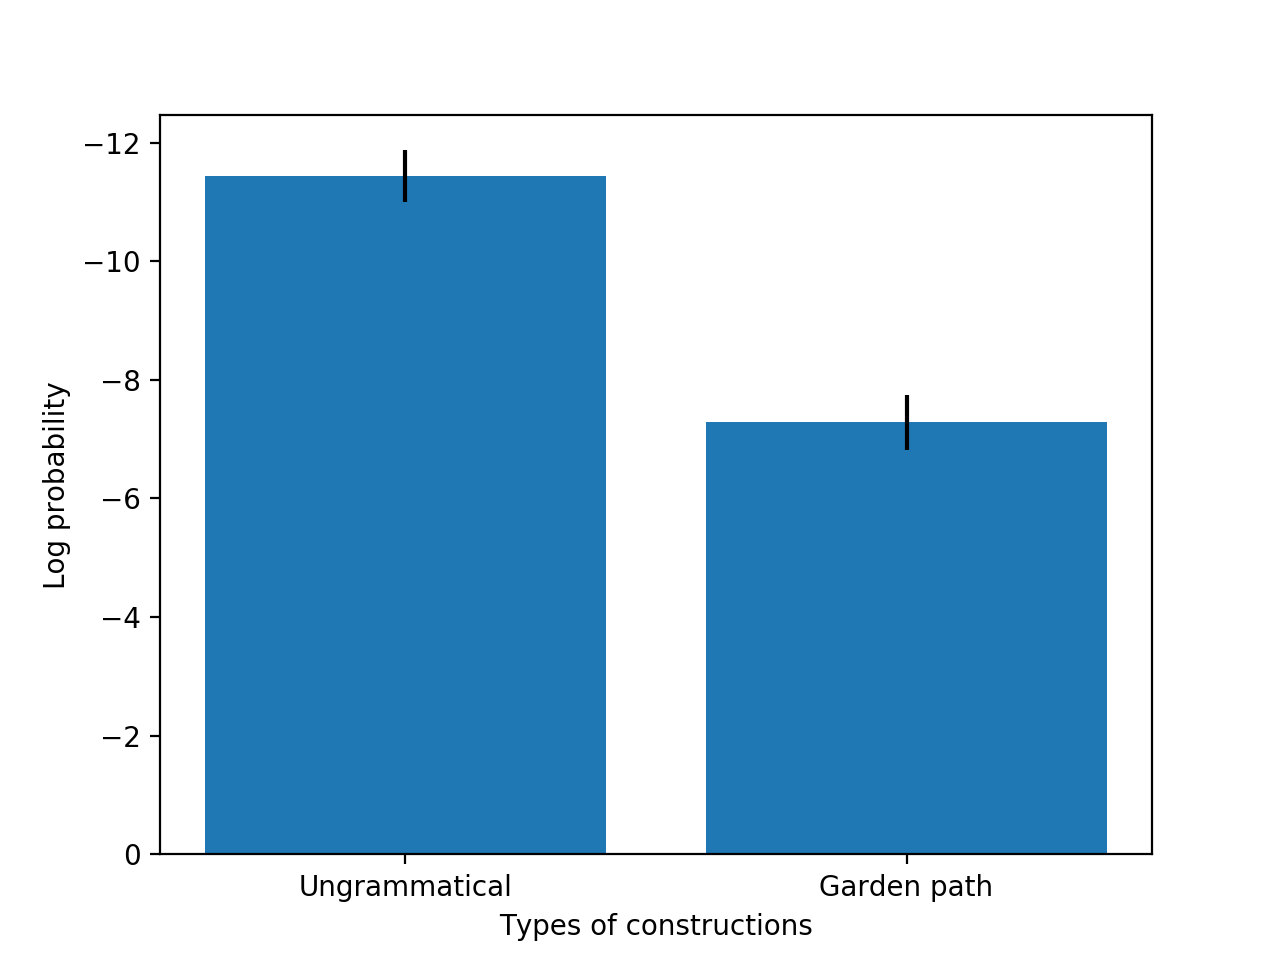
\includegraphics[keepaspectratio,width = \linewidth]{transition_prob.png}

\subsubsection*{4. Does BERT disprefer indefinite nouns or long nouns as the recipient in DO constructions?}
We calculated the probability of a sentence in the following way.  We calculated the probability of each word by shifting the mask one at a time, and make sure that the model does not use the information of words that occur later.  Then, the log probability of a sentence was calculated by adding the log probabilities for each word.\\
e.g.\\
$[[$SEP$]$, the, man, brought, $[$MASK$]]$\\
$[[$SEP$]$, the, man, brought, a, $[$MASK$]]$\\
$[[$SEP$]$, the, man, brought, a, woman, $[$MASK$]]$\\
$[[$SEP$]$, the, man, brought, a, woman, the, $[$MASK$]]$\\
$[[$SEP$]$, the, man, brought, a, woman, the, box, $[$MASK$]]$\\
The log likelihood ratio
$$\text{ln}\frac{\text{P(Verb} | \text{DO)}}{\text{P(Verb} | \text{PD)}}$$
were calculated for each sentence under eight conditions (All examples below are for DO constructions).\\
1. Alternating verbs with pronoun recipient\\
ex. $[$SEP$]$ the man brought her the box . $[$SEP$]$\\
2. Non-alternating verbs with pronoun recipient\\
ex. $[$SEP$]$ the man dropped her the news . $[$SEP$]$\\
3. Alternating verbs with definite recipient\\
ex. $[$SEP$]$ the man brought the friend the box . $[$SEP$]$\\
4. Non-alternating verbs with definite recipient\\
ex. $[$SEP$]$ the man dropped the friend the news . $[$SEP$]$\\
5. Alternating verbs with indefinite recipient\\
ex. $[$SEP$]$ the man brought a friend the box . $[$SEP$]$\\
6. Non-alternating verbs with indefinite recipient\\
ex. $[$SEP$]$ the man dropped a friend the news . $[$SEP$]$\\
7. Alternating verbs with long recipient\\
ex. $[$SEP$]$ the man brought the friend from childhood the box . $[$SEP$]$\\
8. Non-alternating verbs with long recipient\\
ex. $[$SEP$]$ the man dropped the friend from childhood the news . $[$SEP$]$\\
9. Alternating verbs with long indefinite recipient\\
ex. $[$SEP$]$ the man brought a friend from childhood the box . $[$SEP$]$\\
10. Non-alternating verbs with long indefinite recipient\\
ex. $[$SEP$]$ the man dropped a friend from childhood the news . $[$SEP$]$\\
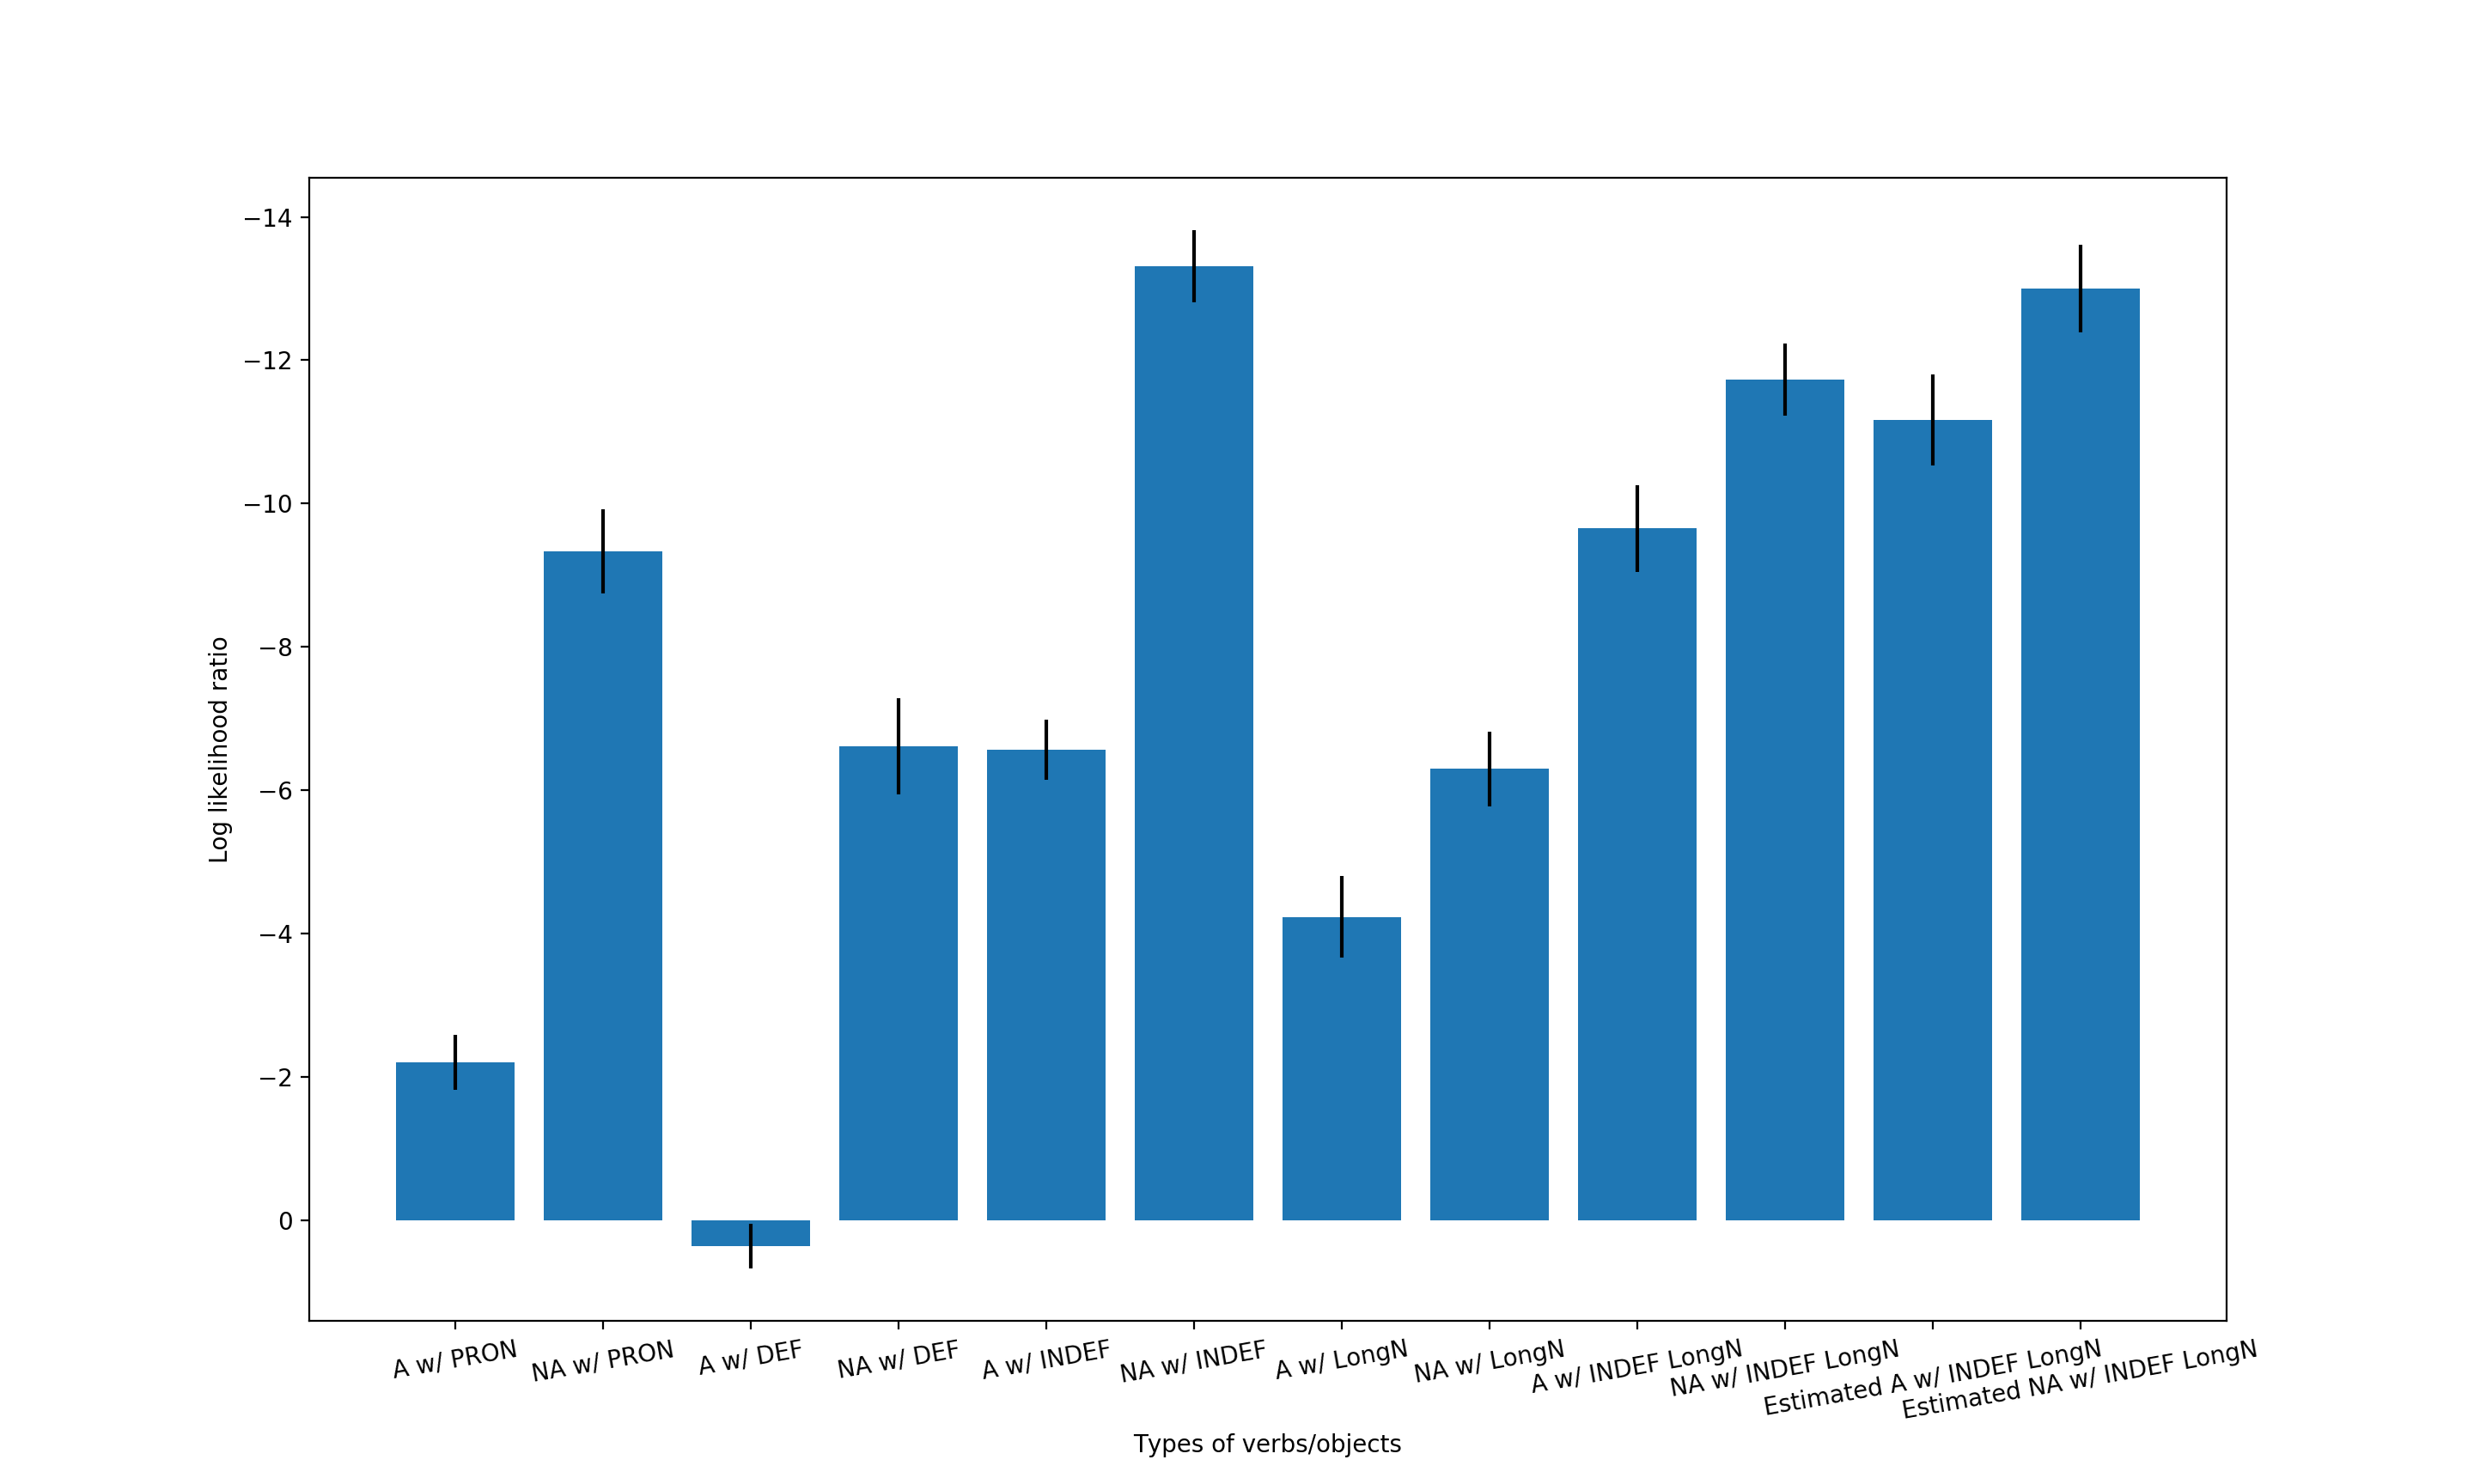
\includegraphics[keepaspectratio,width = \linewidth]{sent_probs_new.png}
A and NA stand for alternating and non-alternating verbs respectively.  The recipients with ``the" had more DO preference than the pronoun recipients.  The long recipients did not have effect on non-alternating verbs.  The long recipients with ``a" had slightly smaller effects than the effects of length and indefiniteness combined.
\subsubsection*{5. Does BERT use lexical semantics?}
Different constructions predict different verbs:\\
$[$SEP$]$ the man $[$MASK$]$ her the credit . $[$SEP$]$\\
gave		-0.033111535012722015\\
offered	-4.356208801269531\\
owed	-4.852931022644043\\
gives		-5.680615425109863\\
handed	-6.4764909744262695\\
$[$SEP$]$ the man $[$MASK$]$ her the paintings . $[$SEP$]$\\
showed	-0.4681996703147888\\
handed	-1.4759321212768555\\
gave		-3.01723575592041\\
brought	-3.482048988342285\\
$[$SEP$]$ the man $[$MASK$]$ her the debt . $[$SEP$]$\\
owed	-0.03584069386124611\\
owes		-3.659550428390503\\
paid		-5.4880242347717285\\
owe		-5.631679058074951\\
owing	-8.58010482788086\\
\textcolor{red}{\textbf{We need a way to quantify this.}}\\
However, it does not seem to distinguish the head in a compound noun.  We calculated the verb predictions for constructions such as\\
$[$SEP$]$ the man $[$MASK$]$ her the karate medal . $[$SEP$]$\\
and compared the distribution with the ones for\\
$[$SEP$]$ the man $[$MASK$]$ her the karate . $[$SEP$]$\\
and\\
$[$SEP$]$ the man $[$MASK$]$ her the medal . $[$SEP$]$\\
Specifically, we calculated the KL divergence of the first distribution from the other two distributions.
If BERT understands the head of the compound noun, then the second divergence should be smaller.  However, there was no significant difference in divergence.\\
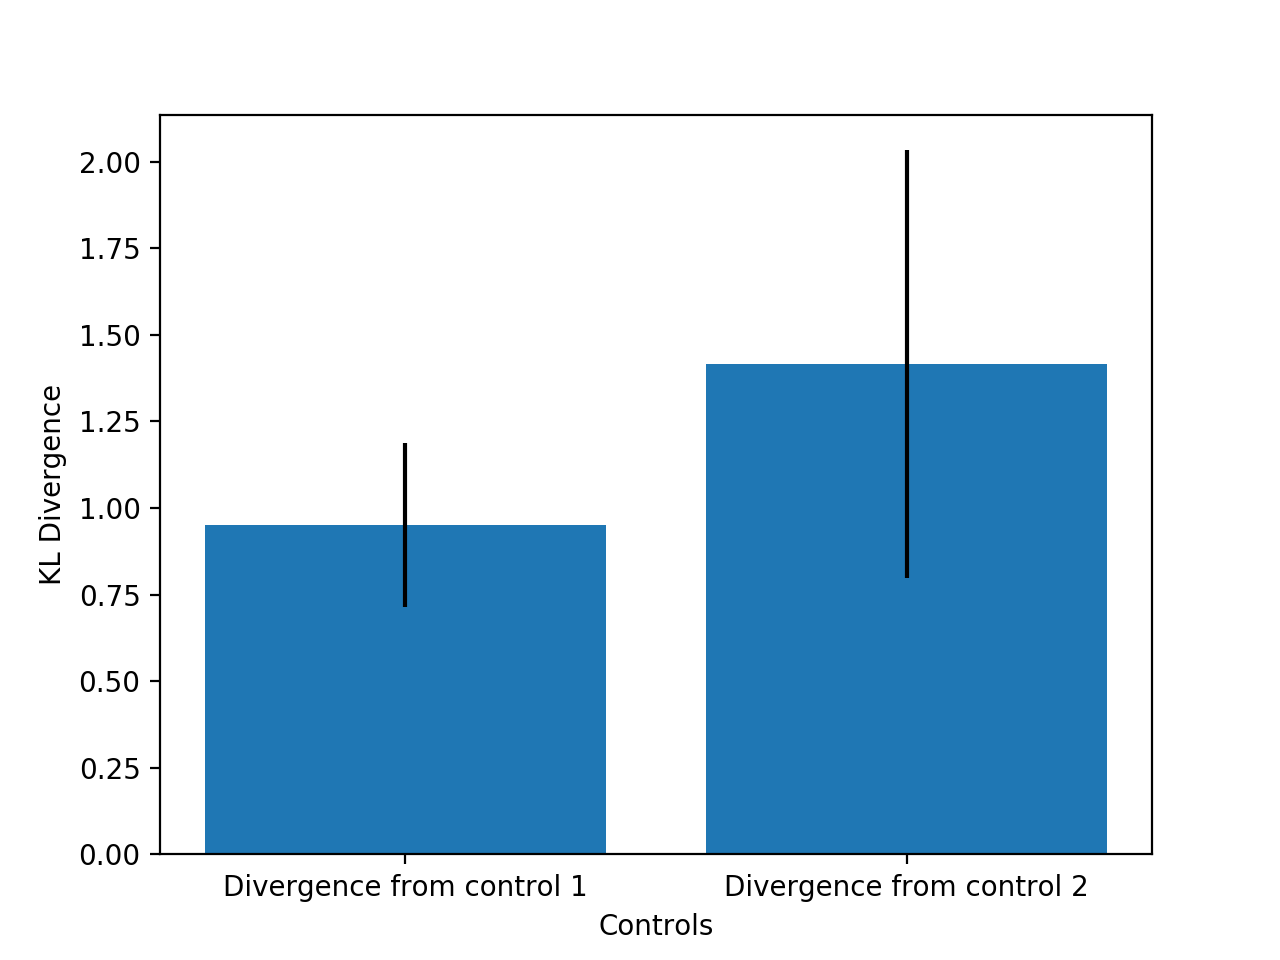
\includegraphics[keepaspectratio,width = \linewidth]{const_divergence.png}
Different verbs predict difference prepositions:\\
$[$SEP$]$ the man put the box $[$MASK$]$ the desk . $[$SEP$]$\\	
on	-0.021063432\\
onto	-4.705445766\\
behind	-6.341177464\\
beside	-6.380657673\\
upon	-6.507708073\\
$[$SEP$]$ the man moved the box $[$MASK$]$ the desk . $[$SEP$]$\\	
across	-1.505526662\\
to	-1.767886281\\
off	-2.062822342\\
from	-2.54642868\\
onto	-2.629494667\\
$[$SEP$]$ the man stole the box $[$MASK$]$ the desk . $[$SEP$]$\\	
from	-0.490429968\\
off	-0.960805058\\
on	-6.614379883\\
under	-7.473587036\\
behind	-7.645296097\\
\textcolor{red}{\textbf{We need a way to quantify this.}}
\subsubsection*{6. Does BERT predict more than alternations?}
We used two double-mask sentences.  The first one we had \\
$[$SEP$]$ the man $[$MASK$]$ him a $[$MASK$]$ . $[$SEP$]$\\
gave	look\\
shot	smile\\
handed	beer\\
offered	nod\\
flashed	grin\\
For the second one, we had\\
$[$SEP$]$ the man $[$MASK$]$ it $[$MASK$]$ them . $[$SEP$]$\\
threw	to\\
handed	for\\
held	from\\
took	at\\
tossed	on\\
\textcolor{red}{\textbf{We need a way to find the joint probability.}}
\subsubsection*{7. Does BERT recognize preferences in who and what questions?}
People prefer saying\\
Who did the man give the book to?\\
than saying\\
Who did the man give the book?,\\
while they do not have preferences between\\
What did the man give to him?\\
and\\
What did the man give him?.\\
In fact, there was a significant difference in DO preferences between who/what questions.\\
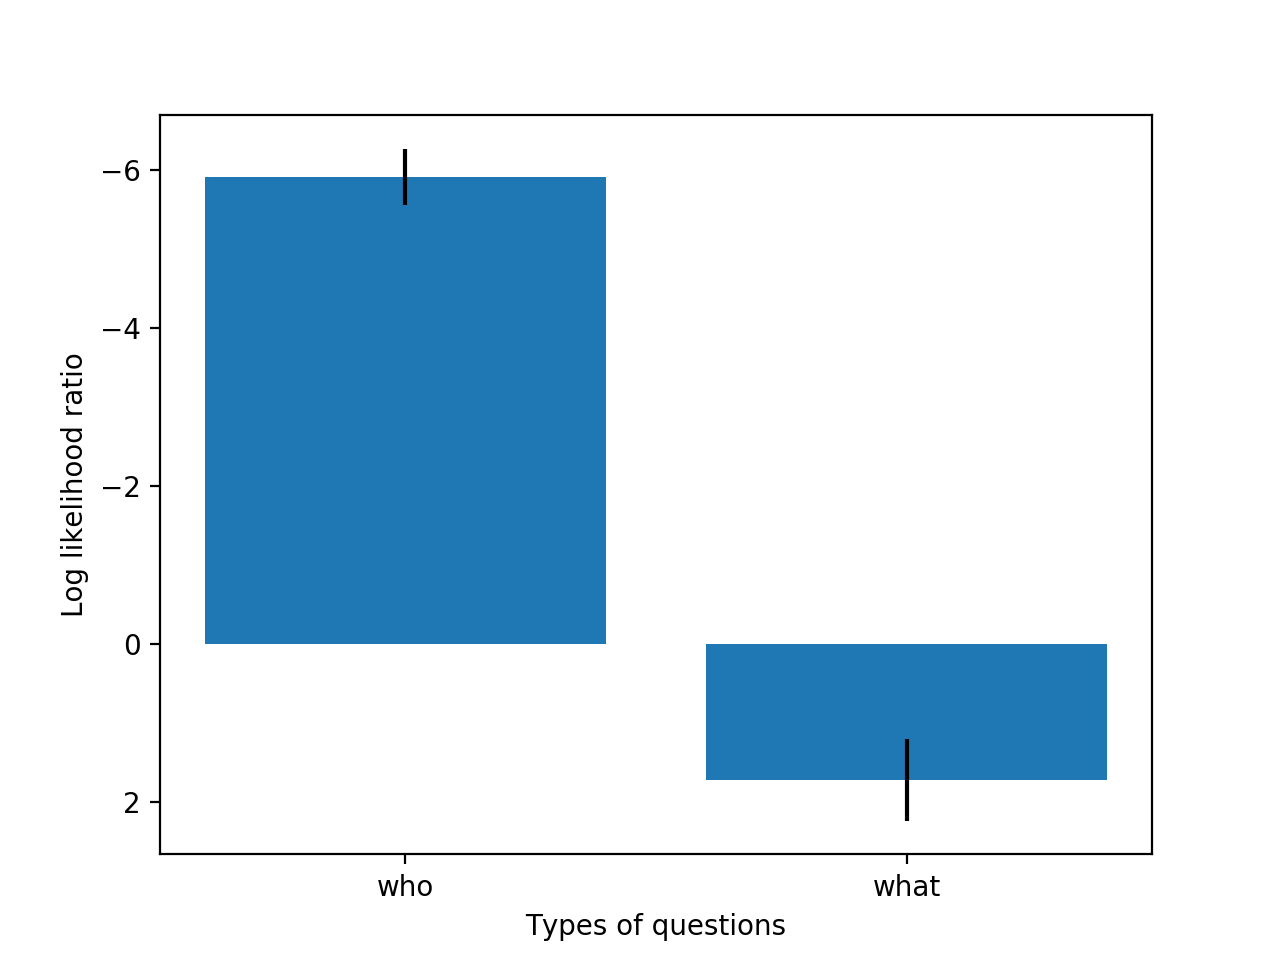
\includegraphics[keepaspectratio,width = \linewidth]{question_new.png}
\subsubsection*{8. Does BERT recognize preferences in passive sentences?}
I compared\\
$[$SEP$]$ the man was brought the box . $[$SEP$]$\\
type sentences and\\
$[$SEP$]$ the box was brought the man . $[$SEP$]$\\
type sentences.  Although these two types of sentences have the same length, the sentence probabilities showed significant differences.\\
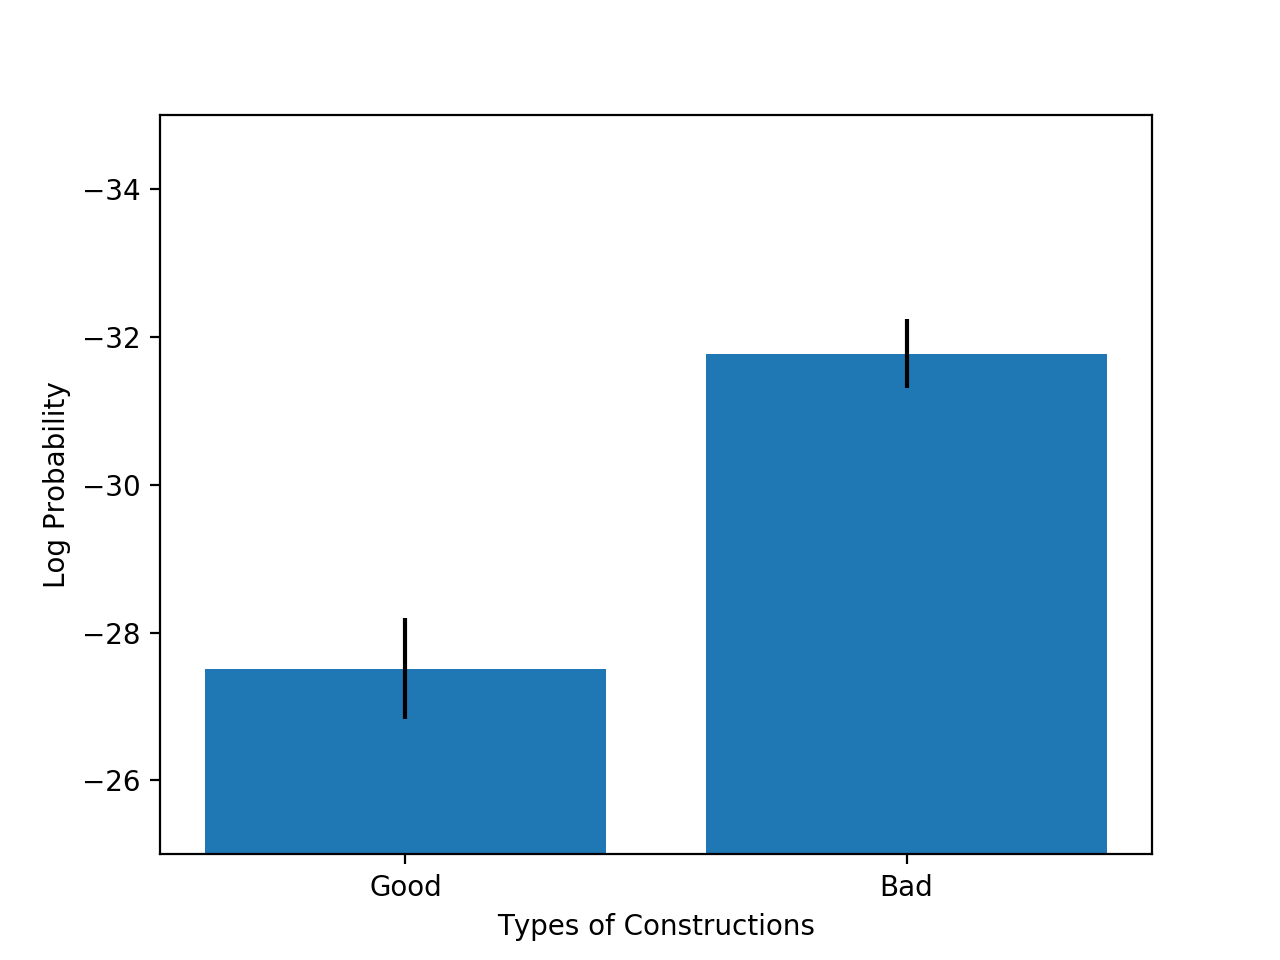
\includegraphics[keepaspectratio,width = \linewidth]{passive_new.png}







\end{document}